\chapter{Diffusion models}
\label{ch:diffusion}

Diffusion models, or DMs~\citep{sohl2015deep,ho2020denoising,nichol2021improved,song2020score}, are defined using two stochastic processes. One, the ``forward'' diffusion process (or ``noising'' process) adds progressively more Gaussian noise to data until it is indistinguishable from a sample from a Gaussian distribution. The other is its inverse: a ``reverse'' (or ``generative'') process which uses a learned ``denoising'' function in the form of a neural network to gradually remove noise from data. Sampling from a DM begins with drawing a sample from a Gaussian distribution that approximates a heavily noised sample from the data distribution. Running the reverse/generative process on this sample then gradually removes noise from it, moving the sample closer to the data manifold. By the end of the generative process, if all is trained well, samples from this process should follow the data distribution. As we will show later, fitting the DM simply involves training a neural network to predict clean data give noisy data using a mean-squared error loss.  We begin by describing in more detail how to sample from a diffusion model before describing how to train one.

\section{Sampling from a diffusion process}

\begin{figure}
    \centering
    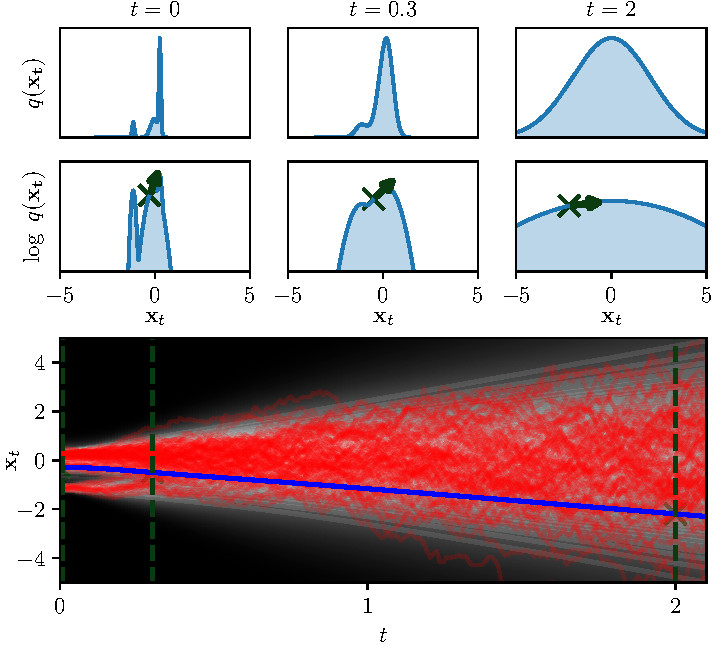
\includegraphics[scale=1]{figs/thesis/diffusion_process.pdf}
    \caption{An example diffusion process for the data distribution $q(\rvx_0)$ shown at the top left. We use $g(t) := \sqrt{2t}$ so that $\sigma_t = t$. \textbf{Top row:} The data distribution $q(\rvx_0)$ and marginals $q(\rvx_t)$ for $t=0.3$ and $t=2$. These marginals are the convolution of the data distribution with a Gaussian distribution of standard deviation $\sigma = t$. For $t=2$, the distribution looks near-Gaussian. \textbf{Middle row:} The distributions from the top row shown in log-space. The green tangent arrows represent $\nabla_{\rvx_t} \log q(\rvx_t)$, the score functions that a neural network would be trained to estimate. \textbf{Bottom row:} The continuous evolution of the forward process for all $t$ between $0$ and $2$. The marginals plotted in the top rows correspond to the ``slices'' made by the dashed green lines. Each faded white line marks a percentile of the $q(\rvx_t)$. The red lines are stochastic trajectories sampled with the SDE described in \cref{sec:diffusion-forward-sde}. The blue line is sampled with the ODE described in \cref{sec:diffusion-ode} and parameterised with the score estimates from the second row.}
    \label{fig:diffusion-overview}
\end{figure}


\begin{table*}
  \caption{Definitions for symbols used.}
  \label{tab:notation}
  \centering
  \begin{tabular}{rp{8cm}}
    \toprule
    Symbol    & Definition   \\
    \midrule
    $\rvx$                                  & Data which we wish to learn a generative model of. \\
    $\rvy$                                  & Data on which the generative model should be conditioned. \\
    $\pdata(\rvx, \rvy)$                    & Data distribution. \\
    \midrule
    $t$                                     & Time in relation to the diffusion SDE and ODE.  \\
    $\rvx_t$                                & ``Noisy'' data at time $t \geq 0$ in the diffusion process.  \\
    $q(\rvx,\rvy,\rvx_{t_1},\ldots,\rvx_{t_n})$   & Joint distribution defined by the data distribution and forward SDE for any $t_1,\ldots,t_n \geq 0$. We will also use $q$ to denote any conditional or marginal of such a distribution.  \\
    $g(t)$                                  & Scaling factor for Wiener process noise added in the forward SDE at time $t$. Defined to be positive for all $t > 0$. \\
    $\sigma(t)$                             & Given by $\sigma(t)^2 = \int g(t)^2 \mathrm{d}t$. Standard deviation of noise added by the forward SDE between time $0$ and $t$. \\
    \midrule
    $\sigma$                                & Equivalent to $\sigma(t)$. When it simplifies results, we will define the process explicitly in terms of $\sigma$ instead of using $t$. \\
    $\rvx_\sigma$                           & ``Noisy'' data described in terms of the standard deviation of added noise $\sigma$ instead of the time $t$. Equivalent to $\rvx_t$ for $t$ satisfying $\sigma = \sigma_t$. \\
    $q(\rvx,\rvy,\rvx_{\sigma_1},\ldots,\rvx_{\sigma_n})$   & Equivalent to $q(\rvx,\rvy,\rvx_{t_1},\ldots,\rvx_{t_n})$ if each $\sigma_i = \sigma(t_i)$. This distribution is agnostic to $g(t)$. \\
    SNR                                     & The signal-to-noise ratio, given by $\frac{1}{\sigma^2}$. \\
    \bottomrule
  \end{tabular}
\end{table*}

\subsection{The forward process as an SDE} \label{sec:diffusion-forward-sde}
This forward process is defined through a combination of the initial condition $\rvx_0 \sim \pdata(\cdot)$ and the stochastic differential equation (SDE):\footnote{We describe here the ``variance-exploding'' diffusion process. We generalise to a broader family of forward processes in ..., which require more complex notation.}
\begin{equation} \label{eq:forward-diffusion}
    \mathrm{d}\rvx = g(t) \mathrm{d}\rvw
\end{equation}
defined for all $t \geq 0$, with $\rvw$ being the standard Wiener process, also known as Brownian motion. The rate at which noise is added, $g(t)$, is a hyperparameter. Many choices of $g(t)$ are possible and we will keep this exposition general by not assuming its value. \citet{karras2022elucidating} show that using $g(t) := \sqrt{2t}$ can lead to good final performance and we use this value in the SDE depicted in \cref{fig:diffusion-overview}.

Given a time $t$, the forward process defines a marginal $q_t(\rvx_t)$, which can be viewed as a version of the data distribution corrupted by Gaussian noise. We will usually refer to such distributions as simply $q(\rvx_t)$, dropping the subscript on the $q$ when it can be inferred from context. Similarly, for any finite set of times $t_1,\ldots,t_n$, the forward process defines a joint distribution over all of $\rvx_{t_1},\ldots,\rvx_{t_n}$ and $\rvx$. We will denote such joint distributions as $q(\rvx,\rvx_{t_1},\ldots,\rvx_{t_n})$, and similarly denote marginal or conditional distributions derived from them with $q$, with the specific distribution of interest being clear from variable names. Many conditional distributions that follow from this are tractable, including the distribution over $\rvx_t$ conditioned on $\rvx$:
\begin{equation}
    q(\rvx_t|\rvx) = \gN \left( \rvx_t; \rvx, \sigma(t)^2 \mI \right) \quad \text{where} \quad \sigma(t)^2 := \int_0^t g(t')^2 \mathrm{d}t'.
\end{equation}
If we view the forward process as adding noise to clean data then $\sigma(t)$ can be viewed as the ``noise-to-signal ratio'' of $\rvx_t$ and, if we follow \citet{karras2022elucidating} by setting $g(t) := \sqrt{2t}$ then we have the simple relationship that $\sigma(t) = t$ for all $t\geq0$.

If $t$ is large and correspondingly $\sigma(t)$ is large, $q(\rvx_t|\rvx)$ will be very well approximated by the Gaussian $\gN(0; \sigma(t)^2\mI)$. In particular, we can observe that the KL divergence
\begin{equation}
    \kl{q(\rvx_t|\rvx)}{\gN(0; \sigma(t)^2\mI)} :=\frac{1}{2\sigma(t)^2} \rvx^\top \rvx
\end{equation}
diminishes with $\sigma(t)^2$. This forward process can therefore be used to map from clean data $\rvx$ to data that is arbitrarily well-approximated by a Gaussian. In the next section we will discuss the more challenging problem of how to invert this process, letting us transform samples from a Gaussian into samples from the data distribution.

\subsection{The reverse SDE} \label{sec:diffusion-reverse-sde}
Our aim in this section is to ``invert'' the forward process from the previous section, yielding a way to create clean data from noise. To do so we refer to a result  derived by \citet{anderson1982reverse}, and recalled in the diffusion modelling context by \citet{song2020score}, showing that the reverse of a diffusion process is also a diffusion process. An application of this result to the diffusion SDE in \cref{eq:forward-diffusion}~\citep{song2020score} reveals that the corresponding reverse-time diffusion SDE is
\begin{equation} \label{eq:reverse-diffusion}
    \mathrm{d}\rvx = -g(t)^2 \nabla_\rvx \log q(\rvx_t) \mathrm{d}t + g(t) \mathrm{d}\bar{\rvw}
\end{equation}
with $\bar{\rvw}$ is a standard Wiener process when time flows backwards and $\nabla_\rvx \log q(\rvx_t)$ is the generally intractable score of $q(\rvx_t)$ as defined through the forward process. The task of the neural network in a diffusion model is to estimate $\nabla_{\rvx_t} \log q(\rvx_t)$, and we will see in \cref{sec:diffusion-training} how this is done. Assuming that we have such an estimator, which we call $s_\theta(\rvx_t, t) \approx \nabla_{\rvx_t} \log q(\rvx_t)$, we can define a generative model as follows. Given large $T \in \mathbb{R}^{>0}$, we sample $\rvx_T \sim \gN(\vzero, \sigma(t)^2 \mI)$; then we simulate the SDE
\begin{equation} \label{eq:reverse-diffusion-with-nn}
    \mathrm{d}\rvx = -g(t)^2 s_\theta(\rvx_t, t) \mathrm{d}t + g(t) \mathrm{d}\bar{\rvw}
\end{equation}
from time $t=T$ to $t=0$ with any SDE solver.\footnote{Possible choices include Euler integration~\citep{ho2020denoising} or more complex Runge-Kutta~\citep{grathwohl2018ffjord} solvers.} We will call the distribution over $\rvx$ parameterised by this process $p_\theta^\text{SDE}(\rvx)$. It approximates the data distribution $\pdata(\rvx)$, with any approximation error being due to (1) imperfect fitting of the score function; and (2) the approximation of $q(\rvx_T)$ with a Gaussian. If $T$ is chosen to be large enough, source (1) will dominate. In practice there will also be some approximation error from numerically simulating the SDE, but we consider $p_\theta^\text{SDE}(\rvx)$ to be the distribution achieved with a zero-error SDE integrator.

% Assuming that we have such an estimator, \cref{eq:reverse-diffusion} provides a way to morph from $\rvx_T$ sampled from a Gaussian distribution for some large $T$, to approximate samples from the data distribution $\rvx_0 \sim \pdata(\cdot|\rvy)$. To do so, we only need a tool for integrating SDEs. This can be simple like Euler integration, or may be a more complex Runge-Kutta~\citep{grathwohl2018ffjord} or Heun~\citep{karras2022elucidating} integration method.

\subsection{A reverse ODE} \label{sec:diffusion-ode}
In this section we will describe how to replace the SDE that parameterises our generative model with an ODE. This can make the integration simpler and also enables exact likelihood evaluation given any $\rvx$ as we will describe shortly. \citet{song2020score} show that, for any diffusion process, there exists a deterministic process whose trajectories share the same marginal distributions $\{q(\rvx_t)\}_t$ as the stochastic diffusion process in \cref{eq:reverse-diffusion}. This deterministic process is described by the ODE
\begin{align}
    \mathrm{d}\rvx &= - \frac{1}{2} g(t)^2 \nabla_\rvx \log q(\rvx_t) \mathrm{d}t \label{eq:diffusion-ode} \\
    &\approx - \frac{1}{2} g(t)^2 \nabla_\rvx s_\theta(\rvx_t, t) \mathrm{d}t. \label{eq:diffusion-ode-with-nn}
\end{align}
We can now use the same generative model described in \cref{sec:diffusion-forward-sde} except that we integrate an ODE instead of an SDE. We will call the resulting distribution $p_\theta^\text{ODE}(\rvx)$. Note that this distribution will not necessarily be identical to $p_\theta^\text{SDE}(\rvx)$ if the approximation of the score function is imperfect, but both will approximate the data distribution.

Sampling from our model now involves simply sampling $\rvx_T \sim \gN(\vzero, \sigma(t)^2\mI)$ and then computing $\rvx_0 = f^{T:0}_\theta(\rvx_T)$, where $f^{T:0}_\theta$ is a function that simulates \cref{eq:diffusion-ode-with-nn} from time $T$ to $0$. Importantly, $f^{T:0}_\theta$ is deterministic and, since it comes from the integration of an ODE, invertible. If we assume that $f^{T:0}_\theta$ is also continuously differentiable then we can apply the change of variables rule to find
\begin{equation}
    p_\theta^\text{ODE}(\rvx_0) = p_\theta(\rvx_T) \left| \det \mJ_{f^{T:0}_\theta}(\rvx_T) \right|^{-1}
\end{equation}
where $\det \mJ_{f^{T:0}_\theta}(\rvx_T)$ is the determinant of the Jacobian of $f^{T:0}_\theta$ evaluated at $\rvx_T$. Following \citet{chen2018neural}, this can be efficiently estimated by integrating the trace
\begin{equation}
    \text{Tr}\left( \frac{\partial}{\partial \rvx_t} \left( - \frac{1}{2} g(t)^2 \nabla_\rvx s_\theta(\rvx_t, t) \right)
    \right)
\end{equation}
of the Jacobian of the ``drift'' term in \cref{eq:diffusion-ode-with-nn} along the path of $\rvx_t$ while simulating the ODE. \citet{song2020score} showed that diffusion models can yield state-of-the-art log likelihoods on image data when evaluated in this way.

\subsection{Other SDEs}
We have seen that it is possible to sample from a diffusion model using either an ODE (\cref{eq:diffusion-ode-with-nn}) or the SDE that inverts the forward process (\cref{eq:reverse-diffusion-with-nn}). A downside of sampling with the SDE is that the requirement to add Gaussian noise during integration means that samples taken with few SDE integration steps are typically of poor quality~\citep{song2020denoising,karras2022elucidating}. This is problematic as sampling with few steps, and thus reduced test-time compute, is an important current research problem~\citep{salimans2022progressive,meng2022distillation,esser2024scaling}. On the other hand, when we can take many integration steps, samples from the ODE are poorer than those from the SDE~\citep{song2020denoising}, which \citep{karras2022elucidating} suggest is due to the build-up of errors caused by our approximation of the score function. This suggests that there is a trade-off between using the SDE, avoiding error build-up, and using the ODE, enabling sampling with fewer integration steps.

\citet{karras2022elucidating} suggest a family of SDEs which ``interpolate'' between the discussed ODE and the discussed SDE~\citep{karras2022elucidating}, making it possible to find an optimal trade-off in this regard. To do so, they suggest the following sum of the ODE from \cref{eq:diffusion-ode} with a distribution-preserving Langevin diffusion term, proving that it maintains the same marginal distributions $\{q(\rvx_t)\}_t$ as the SDE and ODE presented so far:
\begin{align}
    \mathrm{d}\rvx &= \underbrace{- \frac{1}{2} g(t)^2 \nabla_\rvx \log q(\rvx) \mathrm{d}t}_\text{Diffusion ODE from \cref{eq:diffusion-ode}} - \underbrace{\beta(t) \sigma(t)^2 \nabla_\rvx \log q(\rvx) \mathrm{d}t + \sqrt{2\beta(t)}\sigma(t)\mathrm{d}\bar{\rvw}}_\text{Langevin diffusion}  \label{eq:diffusion-edm-sde-exact} \\
    &\approx \underbrace{- \frac{1}{2} g(t)^2 \rvs_\theta(\rvx_t, t) \mathrm{d}t}_\text{Diffusion ODE from \cref{eq:diffusion-ode}} - \underbrace{\beta(t) \sigma(t)^2 \rvs_\theta(\rvx_t, t) \mathrm{d}t + \sqrt{2\beta(t)}\sigma(t)\mathrm{d}\bar{\rvw}}_\text{Langevin diffusion} \label{eq:diffusion-edm-sde-approx}
\end{align}
where $\beta(t)$ is a hyperparameter and $\sigma(t) = \int_0^t g(t') \mathrm{d}t'$ is the standard deviation of $q(\rvx_t|\rvx)$ as defined earlier. 
If $\beta(t) = 0$, we recover the ODE from \cref{eq:diffusion-ode}. The Langevin diffusion part of the SDE, active when $\beta(t) > 0$, can be understood as playing a role similar to running a Markov chain Monte Carlo process~\citep{bishop2006pattern} in that it causes the value of $\rvx_t$ to gradually while staying distributed according to $q(\rvx_t)$. The hyperparameter $\beta(t)$ then controls how ``quickly'' these Langevin dynamics are taking place at each time $t$. \citet{karras2022elucidating} posit that the noise added with $\beta(t) > 0$ helps to compensate for inaccuracies of the ODE from the score function estimate. Using values of $\beta(t)$ that are too large, however, will lead to greater inaccuracies since the Langevin dynamics are also only approximate thanks to the imperfect SDE solver and imperfect score function estimates. If $\beta(t) = \frac{g(t)^2}{2 \sigma(t)^2}$, we recover the SDE from \cref{eq:reverse-diffusion}. In practice, \citet{karras2022elucidating} suggest using values that are tuned through experiments for a given diffusion model.


\section{Learning the score function} \label{sec:diffusion-training}

\subsection{Training is agnostic to the mapping between timestep and noise-to-signal ratio}
The objective, when training a diffusion model, is to obtain a good estimate of the score function, $s_\theta(\rvx_t, t) \approx \nabla_{\rvx_t} \log q(\rvx_t)$ for all $t$ of interest so that we can use it to parameterise our SDE or ODE during sampling. Given that $q(\rvx_t) = \int q(\rvx) \gN(\rvx_t; \rvx, \sigma_t^2\mI) \mathrm{d}\rvx$, we can equivalently state our objective as obtaining a good estimate of 
\begin{equation}
\nabla_{\rvx_t} \log q(\rvx_t) = \nabla_{\rvx_t} \log \int q(\rvx) \gN(\rvx_t; \rvx, \sigma(t)^2\mI) \mathrm{d}\rvx
\end{equation}
for all $\sigma(t)$ of interest. We can state this objective purely in terms of $\sigma(t)$ without considering $t$ itself. Therefore, for the rest of this chapter we will consider the problem of learning a score function for given values of $\sigma$ without considering how they relate to $t$. This means that we can re-use the same learned score function estimator even if we decide to change the relationship between $\sigma$ and $t$ by changing the value of $g(t)$ in the forward SDE (\cref{eq:forward-diffusion}). We can therefore disentangle the learning of a diffusion model from the definition of the ODEs and SDEs used to sample from it. To make this clear, in the remainder of this section when we have in mind a particular noise-to-signal ratio $\sigma=\sigma(t)$ and wish to refer to the corresponding variable $\rvx_t$, we will do so without reference to $t$ by simply writing $\rvx_\sigma$. We will also now write the score estimate as $s_\theta(\rvx_\sigma, \sigma)$ so that it takes $\sigma$ as an argument instead of $t$. In the following, we derive an objective for matching $s_\theta(\rvx_\sigma, \sigma)$ to $\nabla_{\rvx_\sigma} \log q(\rvx_\sigma)$~\citep{vincent2011connection,song2019generative}. These scores are the gradients depicted by arrows in \cref{fig:diffusion-overview}.

\subsection{An objective for learning to estimate the score function} \label{sec:score-function-training-objective}

In \cref{sec:diffusion-ode} we described how to compute the likelihoods of data with respect to our diffusion model. One solution to training the diffusion model would be to explicitly optimise this objective. Doing so would maximise the data likelihood under $p_\theta^\text{ODE}$ without necessarily matching $\rvs_\theta(\rvx_t, t)$ to the score function and has been explored in the past, yielding models called continuous normalising flows~\cite{chen2018neural}. Doing so has some downsides, however; one is that we would need to perform sufficiently many sequential network evaluations to accurately integrate the ODE on every training iteration, potentially making training expensive. Another is that training with this objective has previously been found to be unstable on high-dimensional data~\citep{weilbach2020structured}. 

We will instead derive an alternative based on minimising the mean squared error of an estimate of a score function. 
We will call this the diffusion objective, $\gL_\text{DM}$. It mitigates both of the described downsides of the maximum likelihood objective. First, $\gL_\text{DM}$ is cheaper to train with since its possible to obtain an unbiased estimate of it while evaluating the neural network only once on each data point, instead of simulating a full ODE trajectory as is required for the maximum likelihood objective. Second, $\gL_\text{DM}$ is more a stable objective as we will see that it can be framed as a simple mean-squared error. In \cref{sec:diffusion-likelihood} we will revisit the relationship between $\gL_\text{DM}$ and maximum likelihood-based objectives.

% One may ask why, then, we derive the $\gL_\text{ISM}$ objective in \cref{eq:diffusion-loss-all-sigma} instead of directly optimising the likelihood of the training data. One reason is that the exact likelihood is expensive to compute since it requires an entire simulation of the ODE trajectory. In this section we show, however, that an appropriate choice of $\lambda(\sigma)$ turns the objective proposed in \cref{eq:diffusion-loss-all-sigma} into a lower bound on the data likelihood. This enables likelihood-based training with a cheap-to-evaluate training objective.

To learn to estimate the score function, an ideal objective would be the mean-squared error between the neural network's outputs and the desired score function. We call this the score-matching objective $\gL_\text{SM}$,
\begin{align}
    \mathcal{L}_\text{SM}(\theta, \sigma) &= \EX_{q(\rvx_\sigma)} \left[ || \nabla_{\rvx_\sigma} \log q(\rvx_\sigma) - \rvs_\theta(\rvx_\sigma, \sigma) ||_2^2 \right],
\end{align}
but in general $\gL_\text{SM}$ is intractable because we do not have access to $\nabla_{\rvx_\sigma} \log q(\rvx_\sigma)$. We can, however, obtain an unbiased estimate of $\gL_\text{SM}$. To do so we begin by breaking it down as
\begin{align} \label{eq:lsm-expanded}
    \EX_{q(\rvx_\sigma)} \big[ 
    || \rvs_\theta(\rvx_\sigma, \sigma) ||_2^2
    - 2 \left\langle \nabla_{\rvx_\sigma} \log q(\rvx_\sigma),
    \rvs_\theta(\rvx_\sigma, \sigma) \right\rangle \big]
    + C_1
\end{align}
where $C_1 = \EX_{q(\rvx_\sigma)} \left[ || \nabla_{\rvx_\sigma} q(\rvx_\sigma) ||_2^2 \right]$ does not depend on $\theta$. We prove the following in \cref{sec:proof-that-diffusion-does-score-matching}, letting us rewrite the second term of \cref{eq:lsm-expanded} in terms of the tractable score of the Gaussian $q_{\sigma}(\rvx_\sigma|\rvx)$ instead of the intractable score of $q_{\sigma}(\rvx_\sigma)$:
\begin{align}
\allowdisplaybreaks
    &\EX_{q(\rvx_\sigma)} \left[ - 2 \left\langle \nabla_{\rvx_\sigma} \log q(\rvx_\sigma), \rvs_\theta(\rvx_\sigma, \sigma) \right\rangle \right] \nonumber \\
    =& \EX_{q(\rvx, \rvx_\sigma)} \left[ -2 \left\langle \nabla_{\rvx_\sigma} \log q(\rvx_\sigma|\rvx), \rvs_\theta(\rvx_\sigma, \sigma) \right\rangle  \right].
\end{align}
Substituting this identity into $\mathcal{L}_\text{SM}(\theta, \sigma)$ we get
\begin{align}
    \mathcal{L}_\text{SM}(\theta, \sigma) &= \EX_{q(\rvx, \rvx_\sigma)} \big[ 
    || \rvs_\theta(\rvx_\sigma, \sigma) ||_2^2
    \nonumber\\ &\qquad\qquad\qquad
    - 2 \left\langle \nabla_{\rvx_\sigma} \log q(\rvx_\sigma|\rvx), \rvs_\theta(\rvx_\sigma, \sigma) \right\rangle \big] + C_1 \\
    &= \EX_{q(\rvx, \rvx_\sigma)} \big[ 
    || \rvs_\theta(\rvx_\sigma, \sigma) ||_2^2
    \nonumber\\ &\qquad\qquad\qquad
    - 2 \left\langle \nabla_{\rvx_\sigma} \log q(\rvx_\sigma|\rvx), \rvs_\theta(\rvx_\sigma, \sigma) \right\rangle
    \nonumber\\ &\qquad\qquad\qquad
    + || \nabla_{\rvx_\sigma} \log q(\rvx_\sigma|\rvx) ||_2^2 \big] + C_2 \\
    &= \EX_{q(\rvx, \rvx_\sigma)} \big[ 
    || \rvs_\theta(\rvx_\sigma, \sigma) - \nabla_{\rvx_\sigma} \log q(\rvx_\sigma|\rvx) ||_2^2 \big] + C_2
\end{align}
where $C_2 = C_1 - \EX_{q(\rvx, \rvx_\sigma)}\left[ || \nabla_{\rvx_\sigma} q(\rvx_\sigma|\rvx) ||_2^2 \right]$ is another scalar that does not depend on $\theta$. Introducing the analytic score of $q(\rvx_\sigma|\rvx)$,
\begin{equation}
    \nabla_{\rvx_\sigma} \log q(\rvx_\sigma|\rvx) = \nabla_{\rvx_\sigma} \log \gN(\rvx_\sigma; \rvx; \sigma^2\mI) = \frac{\rvx-\rvx_\sigma}{\sigma^2},
\end{equation}
and defining our implicit score-matching loss as $\mathcal{L}_\text{ISM}(\theta, \sigma) := \mathcal{L}_\text{SM}(\theta, \sigma) - C_2$, we get
\begin{align} \label{eq:ism-loss}
    \mathcal{L}_\text{ISM}(\theta, \sigma) &= \EX_{q(\rvx, \rvx_\sigma)} \left[ 
    || \rvs_\theta(\rvx_\sigma, \sigma) - \nabla_{\rvx_\sigma} \log q(\rvx_\sigma|\rvx) ||_2^2 \right] \\
    &= \EX_{q(\rvx, \rvx_\sigma)} \left[  \label{eq:ism-loss-ve}
    || \rvs_\theta(\rvx_\sigma, \sigma) - \frac{\rvx-\rvx_\sigma}{\sigma^2} ||_2^2 \right]
\end{align}
We can therefore train a diffusion model with the simple objective of a mean-squared error loss between the neural network's output and $\frac{\rvx-\rvx_\sigma}{\sigma^2}$.

Recall that, for sampling, we need the score function estimate to be accurate for a range of $\sigma$. In particular, we will consider a range $\sigma_\text{min}$ to $\sigma_\text{max}$, chosen such that $\sigma_\text{min}$ is sufficiently close to zero and $\sigma_\text{max}$ is large enough to make $q(\rvx_{\sigma_\text{max}})$ roughly Gaussian.\footnote{Setting $\sigma_\text{min}$ to exactly zero would cause problems when we divide by $\sigma$, but we can allow it to get arbitrarily close to zero so that $q(\rvx_{\sigma_\text{min}})$ is arbitrarily close to the data distribution.} We need $s_\theta(\rvx_\sigma, \sigma)$ to be a good approximation of the score for all $\sigma$ within this range. We therefore define the diffusion loss $\gL_\text{DM}$ as an an integral of the implicit score matching loss $\gL_\text{ISM}$ over $\sigma$:
\begin{align} \label{eq:diffusion-loss-all-sigma}
    \mathcal{L}_\text{DM}(\theta) &= \int_{\sigma_\text{min}}^{\sigma_\text{max}} \lambda^\rvs(\sigma) \EX_{q(\rvx, \rvx_\sigma)} \left[ 
    || \rvs_\theta(\rvx_\sigma, \sigma) - \frac{\rvx-\rvx_\sigma}{\sigma^2} ||_2^2 \right] \mathrm{d}\sigma
\end{align}
where $\lambda^\rvs(\sigma)$ is a weighting function that controls how much network capacity is spent modelling the score function at each noise level. In order to cheaply obtain a stochastic but unbiased estimate of \cref{eq:diffusion-loss-all-sigma} we can rewrite the integral with an expectation
\begin{align} \label{eq:exp-diffusion-loss-all-sigma}
    \mathcal{L}_\text{DM}(\theta) &= \EX_{u(\sigma)q(\rvx, \rvx_\sigma)} \left[ \frac{\lambda^\rvs(\sigma)}{u(\sigma)} 
    || \rvs_\theta(\rvx_\sigma, \sigma) - \frac{\rvx-\rvx_\sigma}{\sigma^2} ||_2^2 \right] \mathrm{d}\sigma
\end{align}
where $u(\sigma)$ is a distribution over values of $\sigma$ to use during training that should assign positive density to values between $\sigma_\text{min}$ and $\sigma_\text{max}$ and zero to values outside this range. At each training iteration, this loss is typically evaluated by averaging over a batch containing multiple values of $\rvx$ sampled from the dataset, and with one different value of $\sigma \sim u(\cdot)$ for each value of $\rvx$. This ensures that loss estimates for different elements of the batch are uncorrelated and that we need only evaluate $\hat{\rvx}_\theta$ once for each training example.


% In the following we will describes how $\lambda^\rvs(\sigma)$ can be set to yield a lower-bound on the data likelihood, or to maximise perceptual quality.

\subsection{Indirect score function estimation} \label{eq:diffusion-equivalent-parameterisations}
In the previous section we described an objective that trains the neural network to predict the score function $\nabla_{\rvx_\sigma} q(\rvx_\sigma|\rvx) = \frac{\rvx-\rvx_\sigma}{\sigma^2}$ given $\rvx_\sigma$ and $\sigma$ in a way that is optimal in terms of mean-squared error, and showed that the same estimate is also an optimal prediction of $\nabla_{\rvx_\sigma} q(\rvx_\sigma)$. In this section, we show that this estimate can be used to derive estimates of several other quantities that are also optimal in terms of mean-squared error. First, consider the problem of estimating the clean data $\rvx$. To do so, we can rewrite the diffusion loss in \cref{eq:exp-diffusion-loss-all-sigma} as
\begin{align} \label{eq:x0-diffusion-loss}
    \mathcal{L}_\text{DM}(\theta) &= \EX_{u(\sigma)q(\rvx_0, \rvx_\sigma)} \left[ \frac{\lambda^\rvx(\sigma)}{u(\sigma)}
    || (\rvx_\sigma + \sigma^2 \cdot \rvs_\theta(\rvx_\sigma, \sigma)) - \rvx ||_2^2 \right] \\
    &= \EX_{u(\sigma)q(\rvx_0, \rvx_\sigma)} \left[ 
    \frac{\lambda^\rvx(\sigma)}{u(\sigma)}
    || \hat{\rvx}_\theta(\rvx_\sigma, \sigma) - \rvx ||_2^2 \right]
\end{align}
where $\lambda^\rvx(\sigma) := \frac{\lambda^\rvs(\sigma)}{\sigma^4}$ and we define $\hat{\rvx}_\theta(\rvx_\sigma, \sigma) := \rvx_\sigma + \sigma^2 \cdot \rvs_\theta(\rvx_\sigma, \sigma)$. This reveals that, while optimising the mean-squared error estimate of the score function in \cref{eq:diffusion-loss-all-sigma}, we are implicitly also optimising a mean-squared error estimate of $\rvx$ which is given by $\rvx_\sigma + \sigma^2 \cdot \rvs_\theta(\rvx_\sigma, \sigma)$.

Another quantity that is often of interest is $\epsilon$, which can be understood as the unit Gaussian-distributed noise used during reparameterised sampling of $\rvx_\sigma$ given $\rvx$ as $\rvx_\sigma = \rvx + \sigma \cdot \epsilon$. We can therefore write $\epsilon$ as $\frac{\rvx_\sigma-\rvx}{\sigma}$. To obtain the optimal estimate of $\epsilon$, we can rewrite \cref{eq:exp-diffusion-loss-all-sigma} as
\begin{align} \label{eq:epsilon-diffusion-loss}
    \mathcal{L}_\text{DM}(\theta) &= \EX_{u(\sigma)q(\rvx, \rvx_\sigma)} \left[ 
    \frac{\lambda^\epsilon(\sigma)}{u(\sigma)} || -\sigma \cdot \rvs_\theta(\rvx_\sigma, \sigma) - \frac{\rvx_\sigma-\rvx}{\sigma} ||_2^2 \right] \\
    &= \EX_{u(\sigma)q(\rvx, \rvx_\sigma)} \left[ 
    \frac{\lambda^\epsilon(\sigma)}{u(\sigma)} || \hat{\mathbf{\epsilon}}_\theta(\rvx_\sigma, \sigma) - \epsilon ||_2^2 \right]
\end{align}
where $\lambda^\epsilon(\sigma) := \frac{\lambda^\rvs(\sigma)}{\sigma^2}$ and $\hat{\mathbf{\epsilon}}_\theta(\rvx_\sigma, \sigma) := -\sigma \cdot \rvs_\theta(\rvx_\sigma, \sigma)$. It is therefore clear that we can obtain an estimate of $\epsilon$ from a learned score function as $-\sigma \cdot \rvs_\theta(\rvx_\sigma, \sigma)$.

While we have described the perspective of learning an estimator for the score function and then using it to predict these other quantities if required, the problem of training a diffusion model can equally be framed as one of learning an estimator for $\rvx$ or $\epsilon$ using \cref{eq:x0-diffusion-loss} or \cref{eq:epsilon-diffusion-loss} and then, if required, deriving an estimate of the score function from it. Training with any of these losses can be set up to be exactly equivalent if the weighting function is scaled appropriately as in \cref{eq:x0-diffusion-loss,eq:epsilon-diffusion-loss} and the parameterisation of the neural network's output is handled appropriately. In the remainder of this chapter we will describe the loss as an L2 distance between $\rvx$ and $\hat{\rvx}_\theta(\rvx_\sigma, \sigma)$ as it will simplify some derivations. In the remainder of this dissertation, we will consider models trained to predict $\rvx$ in \cref{ch:conditional-diffusion,ch:flexible-diffusion} and the video experiments in \cref{ch:tddm} and models trained to predict $\epsilon$ in \cref{ch:fdm} and in the molecule generation experiments in \cref{ch:tddm}.

\subsection{Weighting the loss to lower-bound data likelihood} \label{sec:diffusion-likelihood}

We now see how the score-matching objective proposed previously can be used to construct a lower-bound on the data likelihood. To do so, we simulate trajectories from the reverse SDE in \cref{eq:reverse-diffusion-with-nn} as follows. We will simulate trajectories from a time corresponding to $\sigma_\text{max}$ to a time corresponding to some $\sigma_\text{min}$ close to zero by discretising this time interval into points labelled $N,\ldots,0$. As in the rest of \cref{sec:diffusion-training}, we will consider only the noise standard deviation and not time itself so we define the points such that the noise standard deviation for point $i$ is
\begin{equation}
    \Sigma[i] = \frac{i}{N}(\sigma_\text{max} - \sigma_\text{min}) + \sigma_\text{min}.
\end{equation}
such that $\Sigma[0] = \sigma_\text{min}$ and $\Sigma[N] = \sigma_\text{max}$. Then, to simulate the reverse SDE, we perform steps $N,\ldots,1$ and at each step $i$ transition from a state with noise standard deviation $\Sigma[i]$ to one with noise standard deviation $P[i] := \Sigma[i-1]$. For brevity in the remainder of this section we will write $\Sigma[i]$ as simply $\sigma$ and $P[i]$ as $\rho$ when the index is clear from the context. This simulation results in a joint distribution over trajectories of
\begin{align} \label{eq:diffusion-reverse-joint-prob}
    p_\theta(\rvx,\rvx_{\Sigma[0]},\ldots,\rvx_{\Sigma[N]}) = p(\rvx_{\Sigma[N]}) \left( \prod_{i=1}^N p_\theta(\rvx_{\rho} | \rvx_{\sigma}) \right) p_\theta(\rvx|\rvx_{\Sigma[0]})
\end{align}
where $p(\rvx_{\Sigma[N]}) = p(\rvx_{\sigma_\text{max}}) = \gN(\rvx_{\sigma_\text{max}}; \mathbf{0}; \sigma_\text{max}^2\mI)$ is a Gaussian approximation of $q(\rvx_{\sigma_\text{max}})$ with no learnable parameters; $p_\theta(\rvx_{\rho} | \rvx_{\sigma})$ is a step parameterised by our score function estimate; and $p_\theta(\rvx|\rvx_{\Sigma[0]}) = p_\theta(\rvx|\rvx_{\sigma_\text{min}})$ is a final ``likelihood'' to remove all noise from data. If the data values are discrete, as image pixel values are, then reducing $\sigma_\text{min}$ can make the contribution of $\log p_\theta(\rvx|\rvx_{\sigma_\text{min}})$ to the log-likelihood arbitrarily close to zero. The ``data likelihood'' is then a marginal of this joint distribution, $p_\theta(\rvx)$, evaluated on our training data. In the following we describe how we can use \cref{eq:diffusion-reverse-joint-prob} to construct a lower-bound on $p_\theta(\rvx)$, before expanding on the form of each $p_\theta(\rvx_{\rho}|\rvx_{\sigma})$.

We start by noting that the forward process yields an analytically tractable form of $q(\rvx_{\Sigma[0]},\ldots,\rvx_{\Sigma[N]}|\rvx)$ which we can express as
\begin{equation}
    q(\rvx_{\Sigma[0]},\ldots,\rvx_{\Sigma[N]}|\rvx) = q(\rvx_{\Sigma[N]}|\rvx) \prod_{i=1}^N q(\rvx_{\rho} | \rvx_{\sigma}, \rvx).
\end{equation}We combine it with \cref{eq:diffusion-reverse-joint-prob} to construct the following lower-bound of $p_\theta(\rvx)$:
\begin{align}
    &\log p_\theta(\rvx) \\
    \geq &\log p_\theta(\rvx) - \kl{q(\rvx_{\Sigma[0]},\ldots,\rvx_{\Sigma[N]}|\rvx)}{p_\theta(\rvx_{\Sigma[0]},\ldots,\rvx_{\Sigma[N]}|\rvx)} \\
    = &\EX_{q(\rvx_{\Sigma[0]},\ldots,\rvx_{\Sigma[N]}|\rvx)} \left[ \log \frac{p(\rvx_{\Sigma[N]}) p_\theta(\rvx|\rvx_{\Sigma[0]}) \prod_{i=1}^N p_\theta(\rvx_{\rho} | \rvx_{\sigma}) ) }{q(\rvx_{\Sigma[N]}|\rvx) \prod_{i=1}^N q(\rvx_{\rho} | \rvx_{\sigma}, \rvx)} \right] \\
    = & -\underbrace{\kl{q(\rvx_{\Sigma[N]}|\rvx)}{p(\rvx_{\Sigma[N]})}}_\text{prior loss} - \underbrace{\EX_{q(\rvx_{\Sigma[0]}|\rvx)} \left[ - \log p_\theta(\rvx|\rvx_{\Sigma[0]}) \right]}_\text{reconstruction loss} - \underbrace{\mathcal{L}_N(\theta, \rvx)}_\text{diffusion loss} \label{eq:full-diffusion-elbo}
\end{align}
where
\begin{align}
    \mathcal{L}_D(\rvx, \theta; N) = \sum_{i=1}^N \EX_{q(\rvx_{\sigma}|\rvx)} \left[ \kl{q(\rvx_{\rho} | \rvx_{\sigma}, \rvx)}{p_\theta(\rvx_{\rho} | \rvx_{\sigma})} \right].
\end{align}
Following \citet{kingma2021variational}, we will call the first term of \cref{eq:full-diffusion-elbo} the ``prior loss''; the second term the ``reconstruction loss''; and the third term the ``diffusion loss''. The prior loss is not improved by optimising $\theta$ but can be made arbitrarily small by choosing large $\sigma_\text{max}$. The reconstruction loss can similarly be made arbitrarily small on discrete data by choosing small $\sigma_\text{min}$. Therefore, given appropriate choices of $\sigma_\text{min}$ and $\sigma_\text{max}$, the lower-bound will be dominated by the diffusion loss $\mathcal{L}_D(\rvx, \theta; N)$. For the remainder of this section we will focus on estimating $\mathcal{L}_N(\theta, \rvx)$.

To evaluate $\mathcal{L}_D(\rvx, \theta; N)$, we first make explicit the form of each of $q(\rvx_{\rho} | \rvx_{\sigma}, \rvx)$ and $p_\theta(\rvx_{\rho} | \rvx_{\sigma})$. From the definition of the forward process, we have that
\begin{align} \label{eq:q-step-pdf}
    q(\rvx_{\rho} | \rvx_{\sigma}, \rvx) &= \frac{q(\rvx_{\rho} | \rvx) q(\rvx_{\sigma} | \rvx_{\rho})}{q(\rvx_{\sigma}|\rvx)} = \frac{\gN(\rvx_{\rho}; \rvx, \sigma_{\rho}^2 \mI) \gN(\rvx_{\sigma}; \rvx_{\rho}, \sigma^2-\rho^2 \mI) }{\gN(\rvx_{\sigma}; \rvx, \sigma_{\sigma}^2 \mI)}
\end{align}
We can exploit the conjugacy of Gaussians to simplify \cref{eq:q-step-pdf} to the Gaussian
\begin{align}
    q(\rvx_\rho|\rvx_\sigma,\rvx) = \gN( \rvx_\rho; \mathbf{\mu}_Q(\rvx_\sigma, \rvx; \rho, \sigma), \sigma_Q^2(\rho, \sigma) \mathbf{I})
\end{align}
where
\begin{align} \label{eq:mu-q}
    \mathbf{\mu}_Q(\rvx_\sigma, \rvx; \rho, \sigma) &:= \frac{\rho^2}{\sigma^2} \rvx_\sigma + \frac{\sigma^2-\rho^2}{\sigma^2} \rvx \\
    \label{eq:sigma-q}
    \text{and}\quad 
    \sigma_Q^2(\rho, \sigma) &:= \frac{\rho^2 (\sigma^2-\rho^2)}{\sigma^2}.
\end{align}

Recall that our objective is minimised by minimising the KL divergence between $q(\rvx_\rho|\rvx_\sigma,\rvx)$ and $p_\theta(\rvx_{\rho}|\rvx_{\sigma})$, so intuitively a sensible parameterisation for $p_\theta(\rvx_\rho|\rvx_\sigma)$ would be as close as possible to the form of $q(\rvx_\rho|\rvx_\sigma,\rvx)$. Since $p_\theta(\rvx_{\rho}|\rvx_{\sigma})$ cannot be a function of $\rvx$, we cannot make them exactly equal. We instead define $p_\theta(\rvx_\rho|\rvx_\sigma)$ so that they are close by copying the form of $q(\rvx_\rho|\rvx_\sigma,\rvx)$ but approximating $\rvx$ using our estimate $\hat{\rvx}_\theta(\rvx_\sigma, \sigma)$, obtained as described in \cref{eq:diffusion-equivalent-parameterisations}:
\begin{align}
    p_\theta(\rvx_{\rho} | \rvx_{\sigma}) &= \gN( \rvx_{\rho}; \mathbf{\mu}_Q(\rvx_\sigma, \hat{\rvx}_\theta(\rvx_\sigma, \sigma); \rho, \sigma), \sigma_Q^2(\rho, \sigma) \mI ).
\end{align}
We can then express the KL divergence as:
\begin{align}
    &\kl{q(\rvx_{\rho} | \rvx_{\sigma}, \rvx)}{p_\theta(\rvx_{\rho} | \rvx_{\sigma})} \\ 
    = &\frac{1}{2 \sigma_Q^2(\rho, \sigma)} || \mathbf{\mu}_Q(\rvx_\sigma, \rvx; \rho, \sigma) - \mathbf{\mu}_Q(\rvx_\sigma, \hat{\rvx}_\theta(\rvx_\sigma, \sigma); \rho, \sigma) ||_2^2 \\
    = &\frac{1}{2 \sigma_Q^2(\rho, \sigma)} || \frac{\sigma^2-\rho^2}{\sigma^2} ( \rvx - \hat{\rvx}_\theta(\rvx_\sigma, \sigma) ) ||_2^2 \\
    = &\frac{\sigma^2-\rho^2}{2 \sigma^2 \rho^2} || \rvx - \hat{\rvx}_\theta(\rvx_\sigma, \sigma) ||_2^2 \\
    % = &\frac{\sigma^2 - \rho^2}{2 \rho^2 \sigma^2} || \rvx - \hat{\rvx}_\theta(\rvx_\sigma, \sigma) ||_2^2 \\
    = &\frac{1}{2} \left( \frac{1}{\rho^2} - \frac{1}{\sigma^2} \right) || \rvx - \hat{\rvx}_\theta(\rvx_\sigma, \sigma) ||_2^2.
\end{align}
Following \citet{kingma2021variational}, we will proceed by introducing the signal-to-noise ratio defined as $\text{SNR}(\sigma) = \frac{1}{\sigma^2}$. We can then write the KL divergence as
\begin{align}
\kl{q(\rvx_{\rho} | \rvx_{\sigma}, \rvx)}{p_\theta(\rvx_{\rho} | \rvx_{\sigma})} = &\frac{1}{2} \left( SNR(\rho) - SNR(\sigma) \right) || \rvx - \hat{\rvx}_\theta(\rvx_\sigma, \sigma) ||_2^2,
\end{align}
and so
\begin{align}
    \mathcal{L}_D(\rvx, \theta; N) = \frac{1}{2} \sum_{i=1}^N \left( SNR(\rho) - SNR(\sigma) \right) || \rvx - \hat{\rvx}_\theta(\rvx_\sigma, \sigma) ||_2^2.
\end{align}
This reveals that the contribution of each denoising step to the log-likelihood is closely related its change to the signal-to-noise ratio. The squared-error term reveals that it is also strongly dependent on the accuracy of the prediction of $\rvx$ given $\rvx_t$. A better lower-bound will be obtained by taking more steps, and changing the signal-to-noise ratio by less in each step. To make this lower-bound agnostic to the number of steps, we can consider the limit where infinitely many steps are taken. To do so, we  follow \citet{kingma2021variational} and replace $\rho$ with $\sigma-\frac{\sigma_\text{diff}}{N}$, where $\sigma_\text{diff} = \sigma_\text{max}-\sigma_\text{min}$. Then, taking the limit as $N \rightarrow \infty$ gives 
\begin{align}
    \mathcal{L}_D(\rvx, \theta; \infty) &= \lim_{N\rightarrow\infty} \frac{1}{2} \sum_{i=1}^N \left[ \left( \frac{\text{SNR}(\sigma-\frac{\sigma_\text{diff}}{N}) - \text{SNR}(\sigma)}{\frac{\sigma_\text{diff}}{N}} \right) || \rvx - \hat{\rvx}_\theta(\rvx_\sigma, \sigma) ||_2^2 \right] \\
    &= \frac{1}{2} \int_{\sigma_\text{min}}^{\sigma_\text{max}} -\text{SNR}'(\sigma) || \rvx - \hat{\rvx}_\theta(\rvx_\sigma, \sigma) ||_2^2 \mathrm{d}\sigma \label{eq:diffusion-elbo}.
\end{align}
We can take an expectation of this loss over $q(\rvx)=\pdata(\rvx)$ and then rewrite it similarly to the $\rvx$-prediction loss in \cref{eq:x0-diffusion-loss}, which gives
\begin{align} \label{eq:diffusion-loss-likelihood}
    \mathcal{L}_D(\theta; \infty) &= \EX_{u(\sigma)q(\rvx_0, \rvx_\sigma)} \left[ 
    \frac{-\frac{1}{2}\text{SNR}'(\sigma)}{u(\sigma)}
    || \hat{\rvx}_\theta(\rvx_\sigma, \sigma) - \rvx ||_2^2 \right].
\end{align}
This form makes it clear that the $\rvx$-prediction loss in \cref{eq:x0-diffusion-loss} is equal to this lower bound on the data log likelihood if we set $\lambda^\rvx(\sigma) := - \frac{1}{2} \text{SNR}'(\sigma) = \frac{1}{\sigma^3}$. For this reason we will define $\lambda^\rvx_{ELBO}(\sigma) := \frac{1}{\sigma^3}$, and similarly define $\lambda^\rvs_{ELBO}(\sigma) := \sigma$ and $\lambda^\epsilon_{ELBO}(\sigma) := \frac{1}{\sigma}$ as the weighting functions for score prediction and $\epsilon$-prediction objectives which correspond to lower-bounds on the data likelihood.

In the interest of presenting as simple a form of the maximum-likelihood objective, we end this section by demonstrating that a change of variables can be used to rewrite our data likelihood $\mathcal{L}_D(\rvx, \theta; \infty)$ more simply as an integral over the signal-to-noise ratio itself. Defining $\text{SNR}_\text{min} = \frac{1}{\sigma_\text{max}}$ and $\text{SNR}_\text{max} = \frac{1}{\sigma_\text{min}}$,
\begin{align}
    \mathcal{L}_D(\rvx, \theta; \infty) &= \frac{1}{2} \int_{\text{SNR}_\text{min}}^{\text{SNR}_\text{max}} || \rvx - \hat{\rvx}_\theta(\rvx_\text{SNR}, \text{SNR}) ||_2^2 \mathrm{d}\text{SNR}. \label{eq:diffusion-integral-dsnr}
\end{align}
In this equation, we use $\rvx_\text{SNR}$ to denote $\rvx_\sigma$ with $\sigma = \frac{1}{\sqrt{SNR}}$ and redefined the function $\hat{\rvx}_\theta$ to take $\text{SNR}$ as an input instead of $\sigma$.


\subsection{Weighting the loss for perceptual quality} \label{sec:diffusion-perceptual-quality}
Optimising the loss in \cref{eq:diffusion-loss-likelihood} to maximise the data likelihood typically yields diffusion models that are very good when evaluated in terms of data likelihood. The likelihood of data under a model, however, does not always correspond well to the quality of samples from the model as perceived by a human. 

For example, in the image domain, the log-likelihood of an image is dominated by high-frequency features rather than low-frequency features. To explain why, see that state-of-the-art lossless compression on the ImageNet dataset at $32\times32$ resolution yields an average of $3.67$ bits per dimension~\citep{sahoo2023diffusion}, or $3.67\times3\times32^2 / 8192 = 1.4$ kB per image, and at $64\times64$ resolution yields an average of 3.83 bits per dimension~\citep{finlay2020train}, or $3.83\times3\times64^2 / 8192 = 5.7$ kB per image. Therefore, $75\%$ of the bits present in the $64\times64$ images represent detail that is sufficiently high-frequency to be removed by downsampling by just a factor of 2. It seems unlikely that $75\%$ of the information that is semantically-important to humans is removed, suggesting that most bits in high resolution images are spent modelling pixel-level detail rather than the semantically-important features.

\begin{figure}
    \centering
    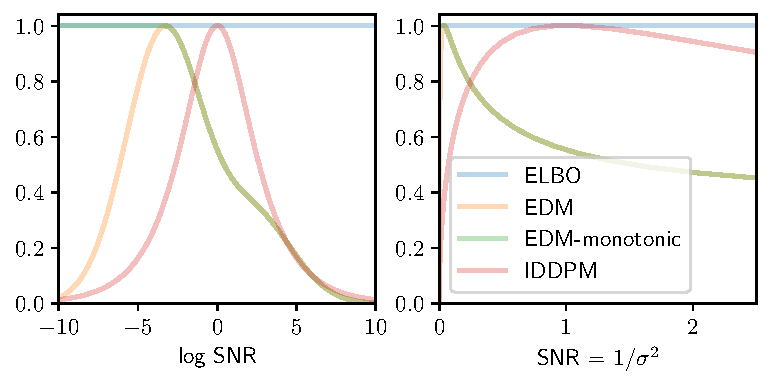
\includegraphics[width=\textwidth]{figs/thesis/diffusion_weighting.pdf}
    \caption{Visualisation of weighting functions $\hat{\lambda}(\sigma)$ plotted against $\log \text{SNR} = \log(1/\sigma^2)$ on the left and against $\text{SNR} = 1/\sigma^2$ on the right. All are normalised to have a maximum value of 1.}
    \label{fig:diffusion-weighting}
\end{figure}

In the diffusion model context, \citet{yang2023diffusion} observed that adding Gaussian noise with even a small standard deviation tends to obscure high-frequency Fourier components of the image, while low-frequency components are not obscured until much more noise is added. This means that, as noise is added during the forward diffusion SDE, high-frequency components will be removed first and low-frequency components will remain until nearer the end. Conversely, while running the reverse SDE to sample from the model, the low-frequency Fourier components are sampled at first, while the amount of noise $\sigma$ is large. Then, as $\sigma$ decreases, increasingly high-frequency components are sampled until the process finishes. We can therefore relate values of $\sigma$ to roughly what Fourier features are sampled being by the diffusion model at that point in the reverse process. If, in order to make samples look perceptually better to humans, we want the diffusion model to be better at generating low-frequency features, we can focus on making the diffusion model obtain better loss for large $\sigma$. This leads us to a common practice in the diffusion model literature: setting the weighting function $\lambda^\rvs(\sigma)$ so that it places relatively greater values on larger values of $\sigma$ than the likelihood-based weighting from \cref{sec:diffusion-likelihood}.

For the remainder of this section, we will describe weighting functions in terms of their difference to the likelihood-based weighting function, as e.g. $\lambda^\rvx(\sigma) = \lambda^\rvx_\text{ELBO}(\sigma) \hat{\lambda}(\sigma)$ where $\lambda^\rvx_\text{ELBO}(\sigma)$ is the likelihood-based weighting for $\rvx$-prediction and $\hat{\lambda}(\sigma)$ is the residual term describing how our weighting corresponds to that. We plot various values of $\hat{\lambda}(\sigma)$ from the literature in \cref{fig:diffusion-weighting}. The likelihood-based weighting, denoted ELBO, has $\hat{\lambda}(\sigma) = 1$. We plot three other choices from the literature. EDM uses $\hat{\lambda}(\sigma) = \gN(-1.2, 1.2^2) \cdot \sigma^2$~\citep{karras2022elucidating,kingma2023understanding} and IDDPM uses $\hat{\lambda}(\sigma) = \text{sech}(\frac{1}{2} \log(1/\sigma^2) )$~\citep{nichol2021improved,kingma2023understanding}. These both have peaks around certain signal-to-noise ratios. EDM-monotonic~\citep{kingma2023understanding} is a variant of EDM designed to be monotonically increasing with $\sigma$ (or decreasing with SNR) so that it always gives higher weight to noisier data.

\section{Using more general diffusion processes}
Many diffusion papers use variations of the forward diffusion SDE we presented in \cref{eq:forward-diffusion} to include a ``drift'' term. Accounting for the drift term adds a small amount of complexity to some of the results presented so far without having a major effect on training or sampling performance in practice~\citep{karras2022elucidating}. Nonetheless, in this dissertation we will present results with diffusion both with and without a drift term so in this section we reiterate all important results for the case where a drift term is included. To start, adding a drift term means modifying the forward SDE,
\begin{equation}
    \mathrm{d}\rvx = g(t) \mathrm{d}\rvw,
\end{equation}
by including the drift term $\rvb_t: \mathbb{R}^n \rightarrow \mathbb{R}^n$, which is a function of the current state $\rvx$:
\begin{align} \label{eq:forward-diffusion-with-drift}
    \mathrm{d}\rvx = \rvb_t(\rvx) \mathrm{d}t + g(t) \mathrm{d}\rvw.
\end{align}
If $\rvb_t(\rvx_t)$ is defined to be zero for all $t$ and $\rvx_t$, this diffusion process is equivalent to that described previously in this chapter. If $\rvb_t(\rvx_t)$ is chosen to be $b_t \cdot \rvx_t$ for some negative scalar $b_t$, there is a negative feedback loop which prevents the value of $\rvx_t$ from growing unboundedly with $t$. In particular, a common choice is to use $\rvb_t(\rvx_t) := - \frac{1}{2}g(t)^2\rvx_t$ which results in what is known as a ``variance-preserving'' diffusion process. The reason for this is that if we assume that $q(\rvx_0)$ (i.e. the data distribution) has unit variance, using $\rvb_t(\rvx_t) := - \frac{1}{2}g(t)^2\rvx_t$ will cause all marginals $q(\rvx_t)$ to similarly have unit variance. See Appendix B of \citet{song2020score} for a proof. Correspondingly, the process that we have described with $\rvb_t(\rvx_t) := 0$ is sometimes called a ``variance-exploding'' diffusion process. The variance of $q(t)$ is simply the sum of the variance of the data distribution and the variance of the added noise $\sigma_t^2 = \int_0^t g(t') \mathrm{d}t'$, and so ``explodes'' as the variance of the added noise grows as $t \rightarrow \infty$.

There are several practical implications of the choice of whether or not to include a drift term. One is in the dynamics of the reverse SDE and reverse ODE. \citet{karras2022elucidating} argue that using a variance-exploding forward diffusion process (i.e. using no drift term) tends to lead to straighter trajectories in the reverse SDE and ODE which are more amenable to simulating with fewer steps, and demonstrate improved performance with few steps in the variance-exploding setting. Another practical implication is in the requirement for normalisation of neural network inputs. Neural networks are usually designed to take inputs that are normalised to have roughly zero mean and unit element-wise variance. Diffusion states $\rvx_t$ will have these properties for all $t$ in a variance-exploding process, but not for large $t$ in a variance-preserving process. This can, though, be handled by appropriately normalising inputs to the neural network.


% One is that, when there is a drift term to ensure that the process is variance-preserving, the process of normalising neural network inputs is simplified. This is because neural networks are usually designed to take inputs that are normalised to have roughly zero mean and unit variance. All $\rvx_t$ will naturally have properties similar to these with a variance-preserving process, as long as the original data distribution had these properties. With a variance-exploding process, care needs to be taken to normalise the inputs to the neural network so that they have roughly unit variance at any time $t$. 

\paragraph{Accounting for the drift term during sampling}
When a non-zero drift term is used, some of the equations derived so far must be modified to account for it. We stuck to the case of a variance-preserving process previously in this chapter to simplify the derivations but analogous results would hold as with a variance-exploding process. In particular, \citet{song2020score} show that our reverse SDE in \cref{eq:reverse-diffusion} becomes
\begin{equation} \label{eq:reverse-diffusion-with-drift}
    \mathrm{d}\rvx = \left( \rvb_t(\rvx) - g(t)^2 \nabla_\rvx \log q(\rvx_t) \right) \mathrm{d}t + g(t) \mathrm{d}\bar{\rvw}
\end{equation}
and our reverse ODE becomes
\begin{align}
    \mathrm{d}\rvx &= \left( \rvb_t(\rvx) - \frac{1}{2} g(t)^2 \nabla_\rvx \log q(\rvx_t) \right) \mathrm{d}t.
\end{align}
That is, the reverse SDE and reverse ODE now both include a $\rvb_t(\rvx)$ term but the other terms are unaltered.

\paragraph{Accounting for the drift term during training}
Our expression for $q(\rvx_t|\rvx)$ becomes
\begin{align}
    q(\rvx_t|\rvx) = \gN(\rvx_t; \alpha(t)\rvx, \sigma(t)^2\mI)
\end{align}
where $\alpha(t) := e^{\int_{0}^t b(t) \mathrm{d}t}$ and $\sigma(t)^2 := \int_0^t g(t')^2 e^{2\int_{t'}^{t} b(t'') \mathrm{d}t''} \mathrm{d}t'$. The score function of a Gaussian with mean $\mathbf{\mu}$ and covariance $\sigma^2\mI$ evaluated at $\rvx$ is $\frac{\mathbf{\mu} - \rvx}{\sigma^2}$ and so the score function of $q(\rvx_t|\rvx)$ becomes $\nabla_{\rvx_t} \log q(\rvx_t|\rvx) = \frac{\alpha(t)\rvx - \rvx_t}{\sigma(t)^2}$. As earlier in this chapter, when we use a variance-exploding process with $\alpha(t) := 1$ the score function simplifies to the expression $\frac{\rvx-\rvx_t}{\sigma(t)^2}$ used previously. We now re-consider our loss function for estimating this score function. We did not rely on the specific properties of the diffusion process to derive the implicit score matching objective from \cref{eq:ism-loss},
\begin{align} \label{eq:ism-loss-with-drift}
    \mathcal{L}_\text{ISM}(\theta, \sigma) &= \EX_{q(\rvx, \rvx_\sigma)} \left[ 
    || \rvs_\theta(\rvx_\sigma, \sigma) - \nabla_{\rvx_\sigma} \log q(\rvx_\sigma|\rvx) ||_2^2 \right],
\end{align}
and so the same derivation still applies. Substituting in the generalised expression for the score function, $\nabla_{\rvx_t} \log q(\rvx_t|\rvx) = \frac{\alpha(t)\rvx - \rvx_t}{\sigma(t)^2}$, yields a new implicit score-matching objective for the diffusion with a drift term:
\begin{align}
    \mathcal{L}_\text{ISM}(\theta, t) &= \EX_{q(\rvx, \rvx_t)} \left[ || \rvs_\theta(\rvx_t, t) - \frac{\alpha(t)\rvx - \rvx_t}{\sigma(t)^2} ||_2^2 \right].
\end{align}
As before, we can integrate $\gL_\text{ISM}$ over a range of $t$ to obtain
\begin{align} \label{eq:general-dm-loss}
    \mathcal{L}_\text{DM}(\theta) &= \EX_{u(t)q(\rvx, \rvx_t)} \left[ \frac{\lambda^\rvs(t)}{u(t)} || \rvs_\theta(\rvx_t, t) - \frac{\alpha(t) \rvx-\rvx_t}{\sigma(t)^2} ||_2^2 \right].
\end{align}
And again we can rewrite the loss with a mean-squared error to $\rvx$ or to $\epsilon$, now defined as $\epsilon := \frac{\rvx_t-\alpha(t)\rvx}{\sigma(t)}$:
\begin{align}
    \mathcal{L}_\text{DM}(\theta) &= \EX_{u(t)q(\rvx, \rvx_t)} \left[ \frac{\lambda^\rvx(t)}{u(t)} || \hat{\rvx}_\theta(\rvx_t, t) - \rvx ||_2^2 \right] \label{eq:diffusion-general-x-prediction} \\
     &= \EX_{u(t)q(\rvx, \rvx_t)} \left[ \frac{\lambda^\epsilon(t)}{u(t)} || \hat{\mathbf{\epsilon}}_\theta(\rvx_t, t) - \epsilon ||_2^2 \right] \label{eq:diffusion-general-epsilon-prediction}
\end{align}
where $\lambda^\rvx(t) := \frac{\alpha(t)^2}{\sigma(t)^4}\lambda^\rvs(t)$; $\hat{\rvx}_\theta(\rvx_t, t) := \frac{\rvx_t + \sigma(t)^2 \cdot \rvs_\theta(\rvx_t, t)}{\alpha(t)}$; $\lambda^\epsilon(t) := \frac{1}{\sigma(t)^2} \lambda^\rvs(t)$ and $\hat{\mathbf{\epsilon}}_\theta(\rvx_t, t) = - \sigma(t) \cdot \rvs_\theta(\rvx_t, t)$.

\paragraph{Computing likelihoods with drift terms}
It is equally possible to lower-bound the data likelihood with a diffusion process that includes a non-zero drift term. We defer to the derivation in \citet{kingma2021variational} since computing the data likelihood is not a core component of this dissertation. Similarly, it is still possible to compute exact likelihoods when a drift term is used in the same manner as described in \cref{sec:diffusion-ode}.